%pictures and spectra
%tables and graphs
%statements of the result

\section{Results}
\label{sec:Results}

Figure \ref{fig:comparison} shows the normalized resistance of the germanium, copper and nickel samples in a temperature range from $\SI{114.286}{\kelvin}$ up to $\SI{451.038}{\kelvin}$.
The normalizing value is the sample specific resitance at $\SI{0}{\celsius}$.

\begin{figure*}
    \centering
    \captionsetup{width=0.9\linewidth}
    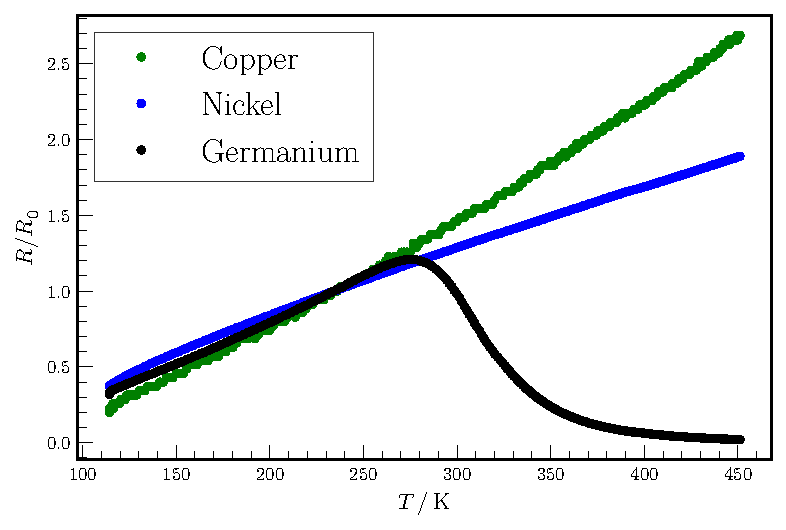
\includegraphics[width=0.7\textwidth]{plots/compare.pdf}
  \caption{Resistance measurement of germanium, copper and nickel, displayed in a nomalized plot based on the resistance at $\SI{0}{\celsius}$.}
    \label{fig:comparison}
\end{figure*}

In figure \ref{fig:metalic-fit} a linear regression in the from
\begin{equation}
    R(T) = R_0 +\beta T
\end{equation}\label{equ:metalic-fit}
has been done and added in the plots. 
As this linear relation describes the metallic behavior, therefore for the semiconductor only the low temperature data up to a temperature of $\SI{260}{\kelvin}$ have been taken into acount.

%% three subfigures next to each others
\begin{figure*}
    \centering
\begin{subfigure}{.45\textwidth}
    \centering
    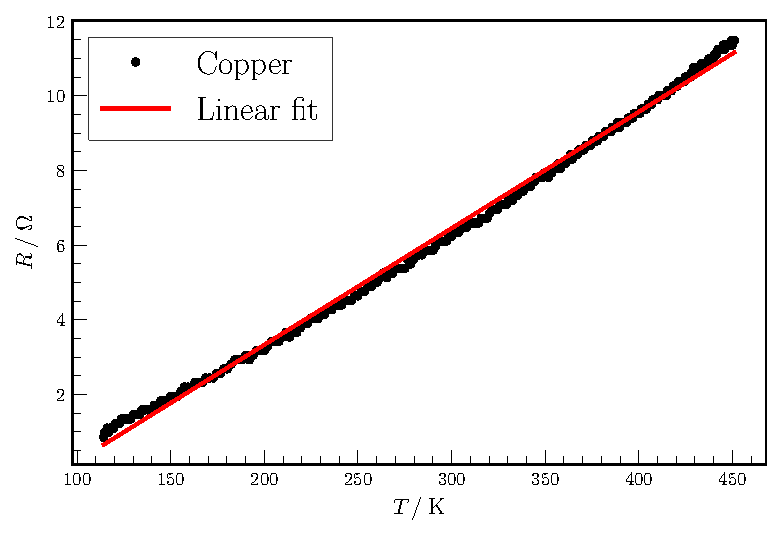
\includegraphics[width=\textwidth]{plots/R2.pdf}
    \caption{Copper}
    \label{fig:Cu}
\end{subfigure}
\begin{subfigure}{.45\textwidth}
    \centering
    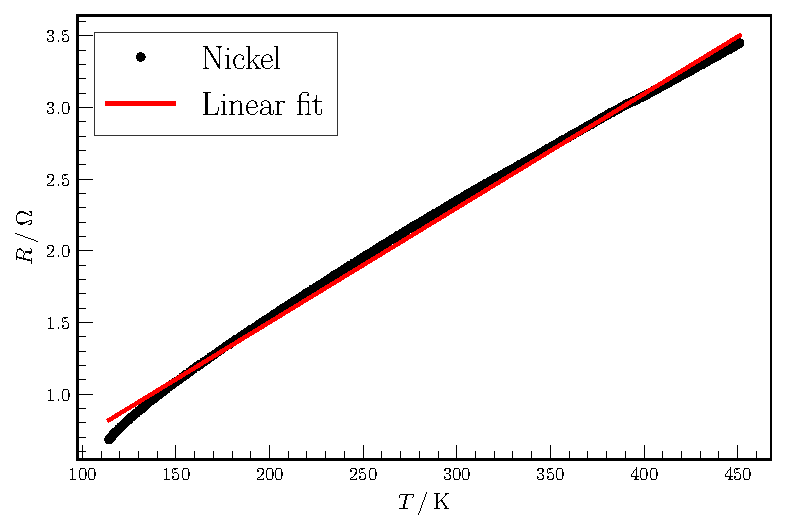
\includegraphics[width=\textwidth]{plots/R3.pdf}
  \caption{Nickel}
    \label{fig:Ni}
\end{subfigure}
\caption{Temperature-dependent resistance of two metallic samples, including a linear regression.}
\label{fig:metallic-fit}
\end{figure*}
%(In the case of germanium only the datapoints with a temperature lower then $\SI{260}{\kelvin}$ have been evaluated.)

The resulting fitting parameters $\beta$ are
\begin{align*}
    \beta(Ge) &= \SI{8.15 \pm 0.04 e-1}{\per\kelvin} \ref{fig:Ge-exp}\\
    \beta(Cu) &= \SI{3.118 \pm 0.001 e-2}{\ohm\per\kelvin} \\
    \beta(Ni) &= \SI{7.966 \pm 0.001 e-3}{\ohm\per\kelvin} \\
\end{align*}\label{equ:results-beta}

For the semiconductor data, up from a temperature of $\SI{304}{\kelvin}$ an exponential fitting 
\begin{equation}
    R(T) = R_0 e^{-B/T} + C
\end{equation}
has been done, which results in the parameters
\begin{align*}
    R_0 &= \SI{9.05 \pm 0.09 e-3}{\ohm} \\
    B &= \SI{-2936 \pm 29 }{\kelvin} \\
    C &= \SI{-4.27 \pm 0.35 }{\ohm} \\
\end{align*} 

Here, $B$ corresponds to $E_g/2k_b$ (compare equation \ref{eq:intrinsic}) so that the bandgap energy is
\begin{equation}
E_g(Ge) = B \times 2 k_b = \SI{0.506 \pm 0.005 }{\eV}.
\end{equation}

\begin{figure*}
    \centering
\begin{subfigure}{.45\textwidth}
    \centering
    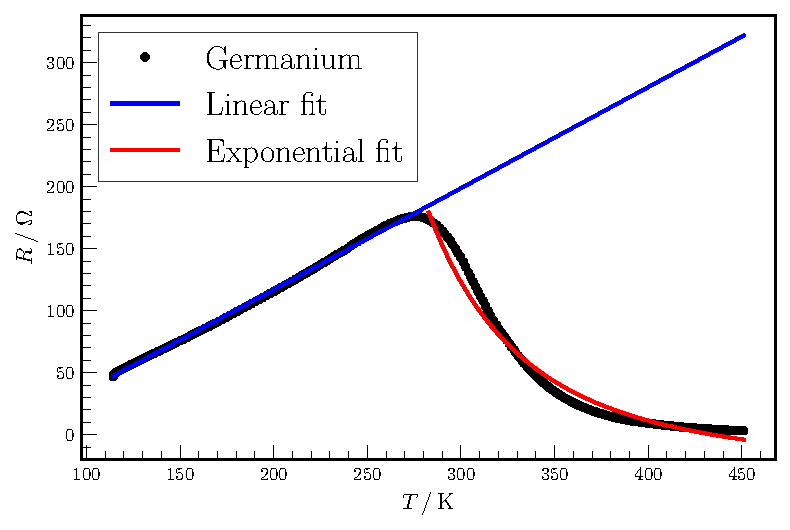
\includegraphics[width=\textwidth]{plots/R1.pdf}
    \caption{Exponential behavior of the resistance for high temperatures higher then $\SI{304}{\kelvin}$.}
    \label{fig:Ge-exp}
\end{subfigure}
\begin{subfigure}{.45\textwidth}
    \centering
    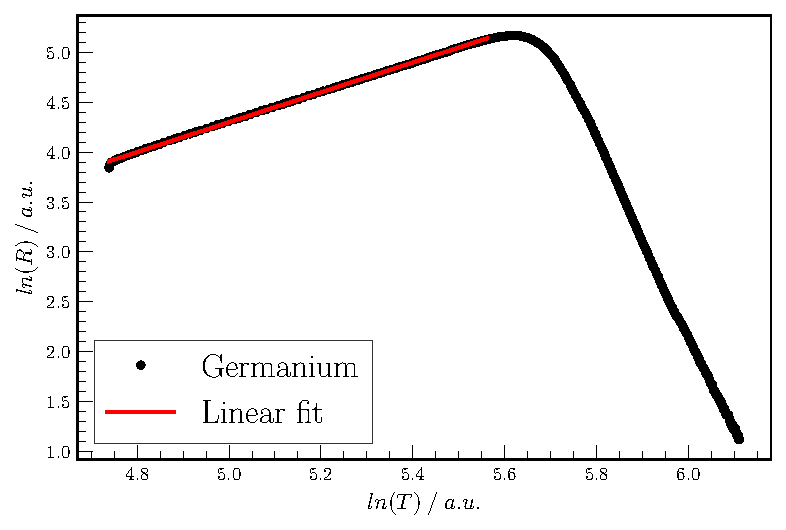
\includegraphics[width=\textwidth]{plots/R1-log.pdf}
  \caption{Double-logarithmic plot with a linear regression for the low temperature regime lower then $\SI{260}{\kelvin}$.}
    \label{fig:Ge-log}
\end{subfigure}
\caption{Temperature-dependent resistance of a germanium sample, with fittings in low and high temperature domain.}
\label{fig:semiconductor-fit}
\end{figure*}

The linear regression in the double-logarithmic plot of resistance against temperature of germanium results in a slope of
\begin{equation}
    \alpha = \num{1.498 \pm 0.004}.
\end{equation}